\documentclass[final]{transcrypto}
\usepackage[utf8]{inputenc}
\usepackage{amsmath}
\usepackage{amsfonts}
\usepackage{amssymb}
\usepackage{float}
\usepackage{caption}
\usepackage{calc}

\usepackage{physics}
\usepackage{amsmath}
\usepackage{tikz}
\usepackage{mathdots}
\usepackage{yhmath}
\usepackage{cancel}
\usepackage{color}
\usepackage{siunitx}
\usepackage{array}
\usepackage{multirow}
\usepackage{amssymb}
\usepackage{gensymb}
\usepackage{tabularx}
\usepackage{booktabs}
\usetikzlibrary{fadings}
\usetikzlibrary{patterns}

%% for code blocks
\usepackage{listings}
\usepackage{xcolor}



\begin{document}
%% Title
\title[RECTANGLE Cipher]{RECTANGLE Cipher}

%% Authors/affiliation:
\author{Abhiram \and Kausheek \and Manu}
\institute{Indian Institute of Technology, Bhilai\\ \email{ambatipudia@iitbhilai.ac.in } \and Indian Institute of Technology, Bhilai\\ \email{akellask@iitbhilai.ac.in} \and Indian Institute of Technology, Bhilai\\ \email{manue@iitbhilai.ac.in}}
\setDOI{}

%% Keywords/abstract:
\keywords{lightweight cryptography \and RECTANGLE \and bit-slice \and survey}
\begin{abstract}
In this paper, we present a survey and our study of block cipher named RECTANGLE. This cipher is a SPN block cipher with 16 ,$4\times 4$ S-Box for substitution and 3 rotations for permutation layer. A strong Sbox which has good hardware performance is chosen. A permutation layer of 3 rotations which provides good diffusion and is fast is used. RECTANGLE is made such that it can be efficiently implemented using bit slicing techniques. As a result it has good performance in both software and hardware. This paper covers overview, specifications, implementations, and attacks on this cipher. We also implemented both versions, bit slicing and normal-one in software (in Rust) and analyzed their performance. A lot of figures are added for easy visualization of the cipher's working and underlying operations.
\end{abstract}
\maketitle
\section{Introduction}
RECTANGLE was proposed as an improved lightweight symmetric cipher that performs well in both software and hardware.\cite{rectangle} Prior to RECTANGLE there were many lightweight ciphers but none of them (except PRESENT which has some security weaknesses)\cite{present} had good performance in both software and hardware. Rectangle uses bit-slice techniques for fast execution; bit-slicing was used in improving software speed of DES and in implementation of Serpant cipher\cite{bit1}\cite{bit2}.

Because of rapidly increasing usage of embedded devices, IoT (Internet of Things) and other things, which require cipher for securing the data that is stored, transmitted and received, there is a huge demand for lightweight cipher\cite{iot}. These devices generally have data that needs to be encrypted with moderately good cipher; using a good secure cipher like AES is not possible because of hardware limitations. These devices often run on low output low power or battery that has small capacity. Also these devices need to be small and fast so small circuits are used. At the time the time RECTANGLE was introduced there were no good lightweight ciphers that had good software performance. There were several good ciphers that had good hardware performance but their software performance is not good. Because of increased usage of lightweight ciphers there was a demand for new lightweight cipher that has good software performance.\cite{sec}

This paper is organized as follows. Section 2 describes the specification of the cipher and algorithm in detail. Section 3 describes bit slice technique. Section 5 describes several attacks on the cipher. Section 6 presents performance of the cipher. Section 7 concludes the paper. Section 8 has nominations for Brownie point.

\section{The Cipher}
Rectangle uses Substitution and Permutation Network (SPN) with each round consisting of S layer of 16 $4 \times 4$ Sbox, P layer of 3 rotations and addition of round key (XOR of state matrix and round key).\\
\newline
Block length: 64 bits\\
Key length: 80 or 128 bits\\
\newline
\textbf{Encryption procedure:}\\
The input is 64 bit plain-text which is written as $4\times 16$ matrix. This matrix represents the "state". This matrix is iterated over several rounds and the initial state of this matrix is given plain-text. And the final "state" matrix is the cipher text. Let the given plain-text be $v_{79}||v_{78}||v_{77}||\dots v_{0}$. Then state matrix will be:
$$S=
\begin{bmatrix}
v_{15} & v_{14} & v_{13} & \dots & v_{2} & v_{1} & v_{0}\\
v_{31} & v_{30} & v_{29} & \dots & v_{18} & v_{17} & v_{16}\\
v_{47} & v_{46} & v_{45} & \dots & v_{34} & v_{33} & v_{32}\\
v_{63} & v_{62} & v_{61} & \dots & v_{50} & v_{49} & v_{48}\\
\end{bmatrix}
$$
We also use the following notation for state matrix:
$$
\begin{bmatrix}
a_{0,15} & a_{0,14} & a_{0,13} & \dots & a_{0,2} & a_{0,1} & a_{0,0}\\
a_{1,15} & a_{1,14} & a_{1,13} & \dots & a_{1,2} & a_{1,1} & a_{1,0}\\
a_{2,15} & a_{2,14} & a_{2,13} & \dots & a_{2,2} & a_{2,1} & a_{2,0}\\
a_{3,15} & a_{3,14} & a_{3,13} & \dots & a_{3,2} & a_{3,1} & a_{3,0}\\
\end{bmatrix}
$$
Where $row_{i} = a_{15,i}||a_{14,i}||a_{13,i}||..a_{0,0}$\\
The algorithm for encryption is as follows:
\begin{center}
\begin{tabular}{c}
\begin{lstlisting}
state = PlainText;
subkey = IV_key;
for i in 0..26 {
    AddRoundKey(state, subkey);
    SubColumn(state);
    ShiftRow(state);
    subkey = NextSubKey(subkey, i);
}
AddRoundKey(state, subkey);
CipherText = state; 
\end{lstlisting}\\
\end{tabular}
\end{center}

There are 25 rounds and a final XOR. Following functions are used in each round:\\
AddRoundKey: State matrix is XORed with round subkey.\\
SubColumn: Each column of state is passed through Sbox (Substitution layer)\\
ShiftRow: Each row of the state is rotated (Permutation layer)\\
NextSubKey: Next round's subkey is obtained using key schedule, see \ref{KeySchedule} for more details.\\
Detailed working of algorithm is described in \ref{Rounds}.
\subsection{Key Schedule}
\label{KeySchedule}
\subsubsection{80 bit key version:}
Make a key state matrix that is $5\times 16$ matrix from the given initial key (KeyIV).\\
Let the given key be $IV = v_{79}||v_{78}||v_{77}||\dots v_{0}$. Then the initial key state matrix will be as follows:
$$
\begin{bmatrix}
v_{15} & v_{14} & v_{13} & \dots & v_{2} & v_{1} & v_{0}\\
v_{31} & v_{30} & v_{29} & \dots & v_{18} & v_{17} & v_{16}\\
v_{47} & v_{46} & v_{45} & \dots & v_{34} & v_{33} & v_{32}\\
v_{63} & v_{62} & v_{61} & \dots & v_{50} & v_{49} & v_{48}\\
v_{79} & v_{78} & v_{77} & \dots & v_{66} & v_{65} & v_{64}\\
\end{bmatrix}
$$
Let us the following notation for elements of the key matrix:
$$
\begin{bmatrix}
k_{0,15} & k_{0,14} & k_{0,13} & \dots & k_{0,2} & k_{0,1} & k_{0,0}\\
k_{1,15} & k_{1,14} & k_{1,13} & \dots & k_{1,2} & k_{1,1} & k_{1,0}\\
k_{2,15} & k_{2,14} & k_{2,13} & \dots & k_{2,2} & k_{2,1} & k_{2,0}\\
k_{3,15} & k_{3,14} & k_{3,13} & \dots & k_{3,2} & k_{3,1} & k_{3,0}\\
k_{4,15} & k_{4,14} & k_{4,13} & \dots & k_{4,2} & k_{4,1} & k_{4,0}\\
\end{bmatrix}
$$
$i^{th}$ row is $row_{i} = k_{15,i}||k_{14,i}||k_{13,i}||..k_{0,0}$\\
\newline
The following operations are applied $i$ times to obtain subkey of $i^{th}$ round:\\
(NextSubKey() function)\\
\begin{enumerate}
    \item S-box is applied to 4 rightmost columns and 4 rows i.e.,
$$k'_{3,i}||k'_{2,i}||k'_{1,i}||k'_{1,i} = Sbox[k_{3,i}||k_{2,i}||k_{1,i}||k_{1,i}]$$ for $i=\{0,1,2,3\}$.
The below figure represents sbox operation. In this figure each block represents 4 bits. After the sbox operation it can be seen that top 4 rows of right most column are darkened because they are modified by the sbox.

\begin{figure}[H]
\caption{Sbox}
\centering
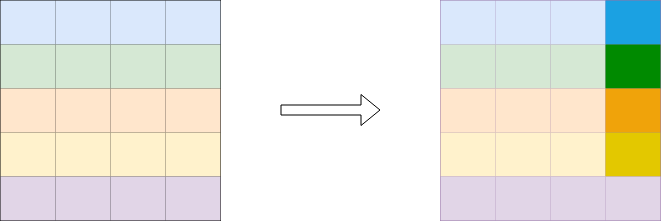
\includegraphics[width=0.85\textwidth]{images/key_s_sbox.png}
\end{figure}
    \item Feistal transformation is applied as follows:\\
\hspace*{0.7cm}$row'_0 = (row_0\ll 8)\oplus row_1$\\
\hspace*{0.7cm}$row'_1 = row_2$\\
\hspace*{0.7cm}$row'_2 = row_3$\\
\hspace*{0.7cm}$row'_3 = (row_3\ll 12)\oplus row_4$\\
\hspace*{0.7cm}$row'_4 = row_0$\\
The below figure shows Feistal transformation. Matrix on the top right is the original matrix with rows circularly rotated by one(downward). Matrix on the left bottom is the original matrix with all rows deleted except 0th and 3rd, which are left shifted by 8 and 12 respectively. (note here each block represents 4 bits)
\newpage
\begin{figure}[H]
\caption{Sbox}
\centering
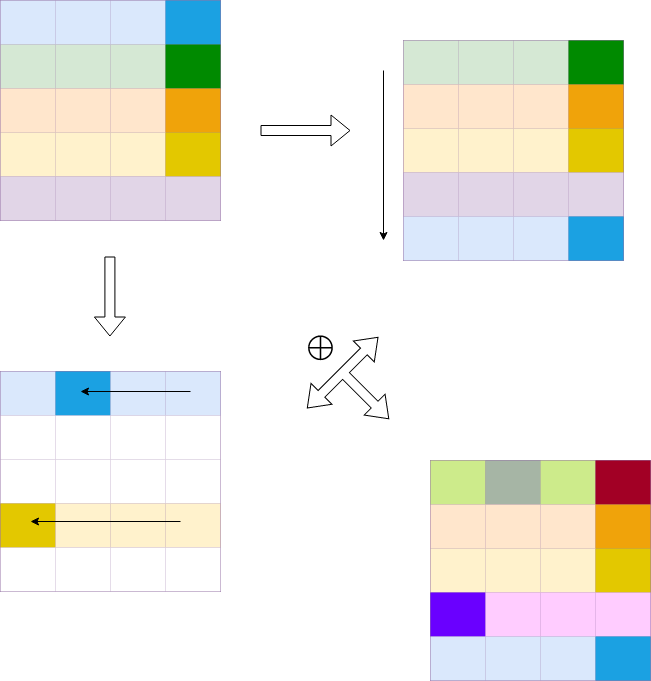
\includegraphics[width=0.85\textwidth]{images/key_s_f.png}
\end{figure}
    \item Last five bits of 0th row  of key-state are XORed with round constant of current round.\\
\begin{figure}[H]
\caption{Sbox}
\centering
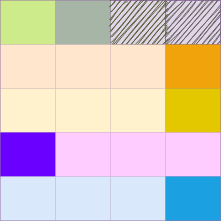
\includegraphics[width=0.26\textwidth]{images/key_s_rc.png}
\end{figure}
\end{enumerate}


\subsubsection{For 128 bit version:}
Procedure for 128 bit is similar to 80 bit with minor differences, here key state matrix is $4\times 32$ matrix instead of $5\times 16$.\\
1. S-box is applied to 8 rightmost columns.\\
2. Feistal transformation is applied as follows:\\
\hspace*{0.7cm}$row_0 = (row_0\ll 8)\oplus row_1$\\
\hspace*{0.7cm}$row_1 = row_2$\\
\hspace*{0.7cm}$row_2 = (row_2\ll 16)\oplus row_3$\\
\hspace*{0.7cm}$row_3 = row_0$\\
3. XOR is same as that in 80 bit version i.e., last five bits of key-state are XORed with round constant of current round.
\subsection{S-box}
\label{sbx}
Only one Sbox is used to reduce the hardware area required. Using more than one Sbox requires increases the hardware area and also doesn't improve security of the cipher. A $4\times 4$ Sbox is very compact in hardware and can be used to make a secure cipher. There are total $16!$ possible $4\times 4$ Sbox and a good Sbox is chosen from these by following a set of mathematical guidelines that make Sbox resistant to linear cryptanalysis, differential cryptanalysis and other attacks.
\begin{table}[H]
	\centering
	\caption{S-box of RECTANGLE}
	\begin{tabular}{|l|l|l|l|l|l|l|l|l|l|l|l|l|l|l|l|l|}
		\hline
 $x$&0&1&2&3&4&5&6&7&8&9&a&b&c&d&e&f\\ \hline
$S(x)$&6&5&c&a&1&e&7&9&b&0&3&d&8&f&4&2 \\ \hline

	\end{tabular}
\end{table}
\subsection{Rounds}
\label{Rounds}
Following operations are applied in each round.\\
\textbf{AddRoundKey}\\
State matrix is XORed with roundkey.\\
(Note: In the following figures used for Rounds section, each block represents one bit)
\begin{figure}[H]
\caption{AddRoundKey}
\centering
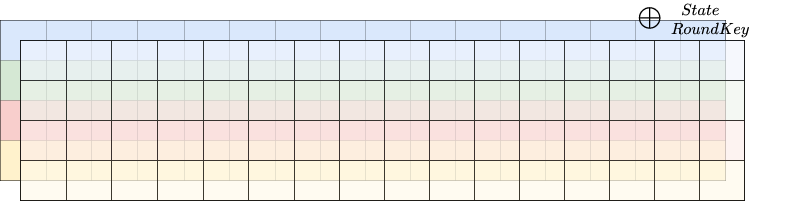
\includegraphics[width=0.85\textwidth]{images/round_xor.png}
\end{figure}
\hspace*{-0.64cm} \textbf{SubColumn}\\
Each column of state is passed through Sbox. This operation (SubColumn) can be efficiently implemented using bit-slicing instead of using Sbox on each column.\\
\begin{figure}[H]
\caption{SubColumn}
\centering
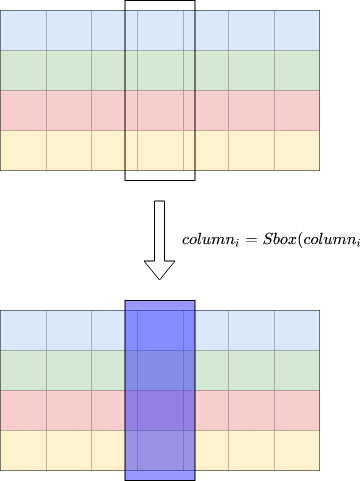
\includegraphics[width=0.45\textwidth]{images/round_sbox.png}
\end{figure}
\hspace*{-0.5cm}\textbf{ShiftRow}\\
0th row is unmodified. 1st row is left (circular) shifted by 1. 2nd row is left (circular) shifted by 12. And 3rd row is left (circular) shifted by 13.\\
\begin{figure}[H]
\caption{ShiftRow}
\centering
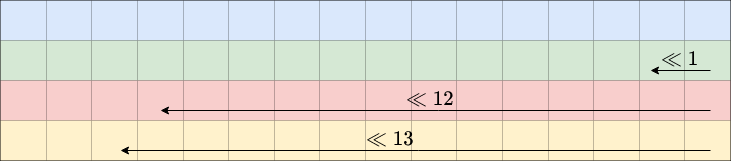
\includegraphics[width=0.85\textwidth]{images/round_shift.png}
\end{figure}
\section{Bit slicing}
SubColumn is significantly faster if bit-slicing techniques are used instead of using lookup table for sbox.
Let $S$ be the state before Subcolumn and $S'$ be the state after applying SubColumn. $T_{1}$, $T_{2}$,..$T_{11}$ are temporary variables. $i$th row of $S$ is 
$A_i$ where $i={0,1,2,3}$ and $i$th row of $S'$ be $B_i$ where $i={0,1,2,3}$\\
Then following 12 steps are calculated for SubColumn to obtain $S'$ from $S$:
\begin{table}[H]
	\begin{tabular}{lll}
1. $T_1=\neg A_1;$  & 2. $T_2=A_0\&T_1;$ & 3. $T_3=A_2\oplus A_3;$ \\
4. $B_0=T_2\oplus T_3;$ & 5. $T_5=A_3|T_1;$  & 6. $T_6=A_0\oplus T_5;$ \\
7. $B_1=A_2\oplus T_6;$ & 8. $T_8=A_1\oplus A_2;$ & 9. $T_9=T_3\&T_6;$ \\
10. $B_3=T_8\oplus T_9;$  & 11. $T_{11}=B_0|T_8;$ & 12. $B_2=T_6\oplus T_{11};$ \\
	\end{tabular}
\end{table}
where "$\neg$" is NOT (negation), "$\&$" is bit-wise AND and "$|$" is bit-wise OR.\\
Also bit-slice implementation is safe against side channel attacks such as cache and timing attacks.\cite{rectanle}
(See \ref{Soft} for details of performance with bit-slicing techniques)
\section{Implementation}
Both bit-slicing and normal versions of RECTANGLE cipher are implemented in Rust (no dependencies).
see "implementations" directory for implementation files. "implementation/RECTANGLE-cipher" contains implementation with bit slicing. And "implementation/without\_bit\_slice" contains implementation without bit slicing. "implementation/timings" contains code used for measuring times/speed of RECTANGLE and  for drawing graphs.
.\section{Cryptanalysis}
\subsection{S-box}
A good (no security weakness) S-box is chosen that has smallest hardware and good hardware performance (See \ref{sbx} for more details). 
\subsection{DDT}
We can see that the Sbox is good as there are no combinations of input-output difference for which there more than 4 pairs.\\
See "attacks" directory for code of DDT (Implemented in python3).
\begin{table}[H]
	\centering
	\caption{DDT of S-box}
	\begin{tabular}{|l||l|l|l|l|l|l|l|l|l|l|l|l|l|l|l|l|}
		\hline
 &  0&	1&	2&	3&	4&	5&	6&	7&	8&	9&	a&	b&	c&	d&	e&	f\\ \hline
 \hline
0& 16 & 0 & 0 & 0 & 0 & 0 & 0 & 0 & 0 & 0 & 0 & 0 & 0 & 0 & 0 & 0 \\ \hline
1& 0 & 0 & 0 & 2 & 0 & 0 & 4 & 2 & 0 & 0 & 0 & 2 & 0 & 0 & 4 & 2 \\ \hline
2& 0 & 0 & 0 & 0 & 0 & 0 & 2 & 2 & 2 & 0 & 2 & 0 & 2 & 4 & 0 & 2 \\ \hline
3& 0 & 0 & 0 & 2 & 0 & 0 & 2 & 0 & 2 & 4 & 2 & 2 & 2 & 0 & 0 & 0  \\ \hline 
4& 0 & 0 & 0 & 4 & 0 & 0 & 0 & 4 & 0 & 0 & 0 & 4 & 0 & 0 & 0 & 4  \\ \hline
5& 0 & 2 & 0 & 0 & 4 & 2 & 0 & 0 & 4 & 2 & 0 & 0 & 0 & 2 & 0 & 0  \\ \hline
6& 0 & 2 & 4 & 0 & 2 & 0 & 0 & 0 & 0 & 0 & 0 & 2 & 2 & 2 & 0 & 2  \\ \hline
7& 0 & 0 & 4 & 0 & 2 & 2 & 0 & 0 & 0 & 2 & 0 & 2 & 2 & 0 & 0 & 2  \\ \hline
8& 0 & 2 & 0 & 2 & 0 & 2 & 0 & 2 & 0 & 2 & 0 & 2 & 0 & 2 & 0 & 2  \\ \hline
9& 0 & 2 & 0 & 0 & 0 & 2 & 4 & 0 & 0 & 2 & 0 & 0 & 0 & 2 & 4 & 0  \\ \hline
a& 0 & 0 & 0 & 0 & 0 & 4 & 2 & 2 & 2 & 0 & 2 & 0 & 2 & 0 & 0 & 2  \\ \hline
b& 0 & 4 & 0 & 2 & 0 & 0 & 2 & 0 & 2 & 0 & 2 & 2 & 2 & 0 & 0 & 0  \\ \hline
c& 0 & 0 & 0 & 0 & 4 & 0 & 0 & 0 & 4 & 0 & 4 & 0 & 0 & 0 & 4 & 0  \\ \hline
d& 0 & 2 & 0 & 0 & 0 & 2 & 0 & 0 & 0 & 2 & 4 & 0 & 0 & 2 & 4 & 0  \\ \hline
e& 0 & 0 & 4 & 2 & 2 & 2 & 0 & 2 & 0 & 2 & 0 & 0 & 2 & 0 & 0 & 0  \\ \hline
f& 0 & 2 & 4 & 2 & 2 & 0 & 0 & 2 & 0 & 0 & 0 & 0 & 2 & 2 & 0 & 0 \\ \hline
	\end{tabular}
\end{table}

\subsection{LAT}
We can see that the Sbox is good as there are no bias values exceeding $\pm 4$.\\
See "attacks" directory for code of LAT (Implemented in Rust).
\begin{table}[H]
	\centering
	\caption{LAT of S-box}
	\begin{tabular}{|l||l|l|l|l|l|l|l|l|l|l|l|l|l|l|l|l|}
		\hline
&0&1&2&3&4&5&6&7&8&9&a&b&c&d&e&f\\ \hline
\hline
0&+8&.&.&.&.&.&.&.&.&.&.&.&.&.&.&.\\ \hline
1&.&.&.&+4&.&-4&.&.&+2&-2&-2&-2&-2&-2&+2&-2\\ \hline
2&.&.&.&.&.&.&+4&+4&.&.&+4&-4&.&.&.&.\\ \hline
3&.&.&.&-4&+4&.&.&.&-2&+2&-2&-2&-2&-2&+2&-2\\ \hline
4&.&.&.&.&.&.&-4&+4&.&.&.&.&.&.&+4&+4\\ \hline
5&.&.&-4&.&.&-4&.&.&-2&+2&-2&-2&+2&+2&-2&+2\\ \hline
6&.&.&.&.&.&.&.&.&+4&+4&.&.&-4&+4&.&.\\ \hline
7&.&.&-4&.&-4&.&.&.&-2&+2&+2&+2&-2&-2&+2&-2\\ \hline
8&.&.&.&-4&-2&-2&+2&-2&.&-4&.&.&-2&+2&+2&+2\\ \hline
9&.&.&.&.&-2&+2&+2&-2&+2&+2&-2&-2&+4&.&+4&.\\ \hline
a&.&.&.&-4&-2&-2&-2&+2&+4&.&.&.&+2&-2&-2&-2\\ \hline
b&.&.&.&.&+2&-2&+2&-2&+2&+2&+2&+2&.&-4&.&+4\\ \hline
c&.&+4&.&.&-2&+2&-2&-2&.&.&.&-4&-2&-2&-2&+2\\ \hline
d&.&+4&+4&.&-2&-2&+2&+2&-2&+2&-2&+2&.&.&.&.\\ \hline
e&.&-4&.&.&-2&+2&+2&+2&.&.&-4&.&-2&-2&-2&+2\\ \hline
f&.&+4&-4&.&+2&+2&+2&+2&+2&-2&-2&+2&.&.&.&.\\ \hline
	\end{tabular}
\end{table}
\subsection{Linear Cryptanalysis}
RECTANGLE is resistant to linear cryptanalysis attacks. Maximum number of rounds that can be attacked using linear cryptanalysis is 14. Also there is no clustering of linear trails which can make effective distinguish-er for more than 15 rounds.\\
These estimations are obtained as follows. If $\epsilon$ is the bias for a liner trail then the correlation contribution is $2\epsilon$. A liner propagation is made of liner trails. Below theorem is used for estimation of correlation potential.\\
\textbf{Theorem 1}. The square of a correlation (or correlation contribution) is called correlation potential.The average correlation potential between an input and an output selection pattern is the sum of the correlation potentials of all linear trails between the input and output selection patterns:
$$E(C_t^2) = \sum (C_i)^2$$ 
where $C_t$ is the overall correlation, and $C_i$ is the correlation coefficient of linear trail.\\
Best linear trails from round 1 to round 15 are obtained using search algorithm(see \ref{diff}). Results of the search program are as follows:\cite{rectangle}\cite{imprAttack}
\begin{enumerate}
    \item There are 128 best linear propagation's with an average correlation potential $1860\times 2^{-80}\approx 2^{-69.14}$ each, which is lower than $2^{-64}$. Each is composed of 891 linear trails. Among the 891 trails, 2 with correlation potential $2^{-74}$ each, 26 with correlation potential $2-{76}$ each, 151 with correlation potential $2^{-78}$ each, and 712 with correlation potential $2_80$ each.
    \item Among all the linear propagation's, the maximum number of trails of a linear propagation is 891. Actually,the best linear propagation's have the maximum number of trails.
\end{enumerate}
Since there are no clustering that can be used to construct a linear propagation, RECTANGLE(25 rounds) is resistant to linear attacks. 
\subsection{Differential Cryptanalysis}
\label{diff}
RECTANGLE is resistant to differential cryptanalysis attacks. Maximum number of rounds that can be attacked using differential cryptanalysis is 18, 18 round distinguish-er(using 14 round different propagation).\\
Since we are using a 64 bit key we need a difference propagation with probability of at-least $2^{-63}$.
The authors of RECTANGLE's paper used a modified version of M. Matsui's search algorithm for finding all differential/linear trials which uses branch and bound method. Best differential trails from round 1 to round 15 are obtained using this algorithm. Results of the search are as follows \cite{rectangle}: 
\begin{enumerate}
 \item here are 32 best difference propagation's with probability $1300\times 2^{-76}\approx 2^{-65.66}$ each. Each is composed of 7 differential trails. Among the 7 trails, one with probability $2^{66}$, two with probability $2^{69}$each,one with probability $2^{72}$, one with probability $2^{75}$, and two with probability $2^{76}$ each.
\item Among all the difference propagation's, the maximum number of trails of a difference propagation is 131,i.e., a difference propagation is composed of at most 131 different differential trails. For such a difference propagation, the probability is $421\times 2^{76}\approx 2^{67.28}$
\end{enumerate}
We can see that there are no difference propagation's that have probability higher than $2^{-63}$ and there is low clustering of trails. Therefore we can not construct a difference propagation for more than 14 rounds. And RECTANGLE(25 rounds) is resistant to differential attacks.
\subsection{Difference Propagation}
Full dependency is reached after 4 rounds and highest rounds that can be attacked are 18, therefore 7 rounds are used as security margin. Following figures show a difference propagation when rightmost bit is altered in 0th row. (Darkened colors means they are affected by the difference)
\newpage
\begin{figure}[H]
\caption{Example Difference propagation 1}
\centering
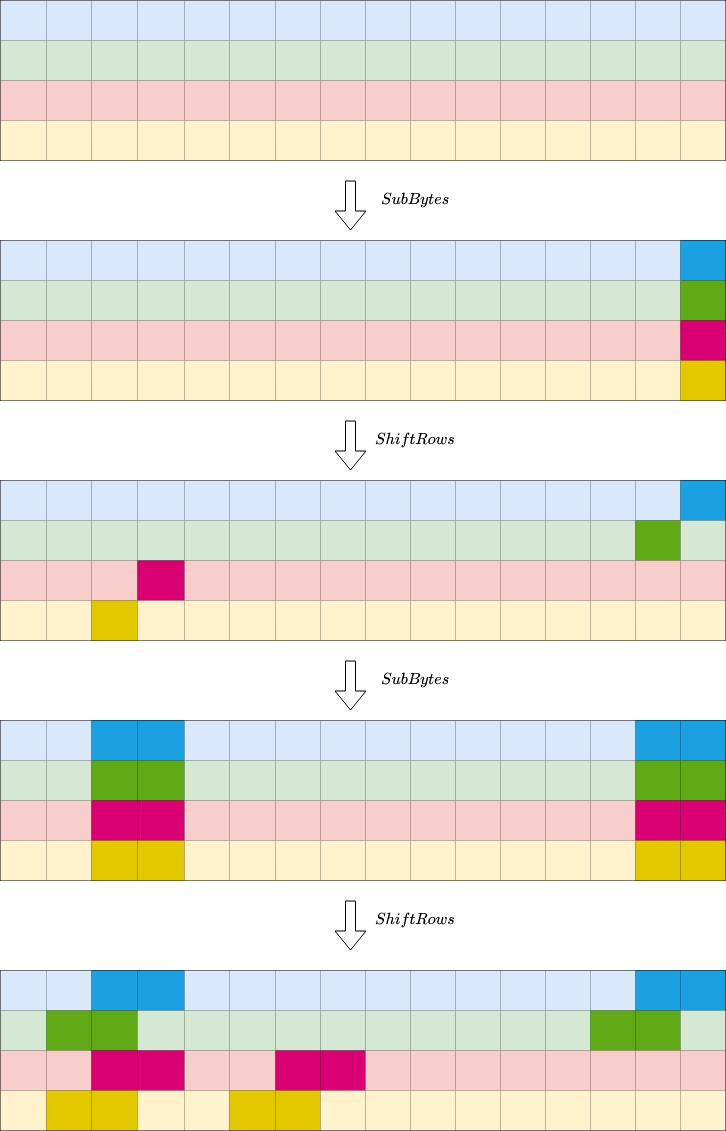
\includegraphics[width=0.85\textwidth]{images/diff_prop1_xor.png}
\end{figure}
\begin{figure}[H]
\caption{Example Difference propagation 2}
\centering
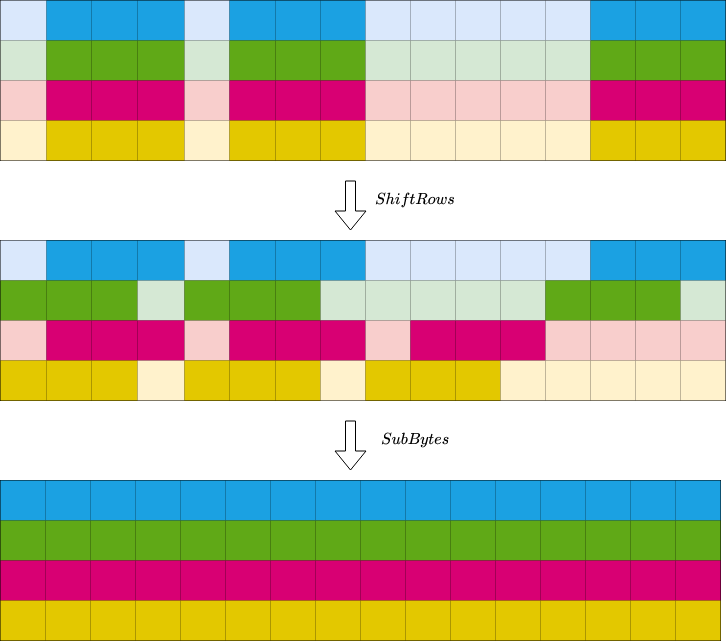
\includegraphics[width=0.85\textwidth]{images/diff_prop2_xor.png}
\end{figure}
\newpage
\section{Performance}
\subsection{Performance with Bit slicing Techniques}
\label{Soft}
Time with bit-slicing: $34.661\pm 1.186\mu $s\\
Time without bit-slicing: $118.429\pm 1.148 \mu $s\\
(for one encryption of 64 bit)\\
Measured with implementation in Rust. These statistics are obtained with implementation running on a machine with Intel Core i5-8250U CPU @ 1.60Ghz x 8, with 8GB memory (DDR4), using Ubuntu 20.04 64 bit (5.4.0-54-generic Linux kernel).
\begin{figure}[H]
\caption{Comparison of RECTANGLE with and without bit-slicing}
\centering
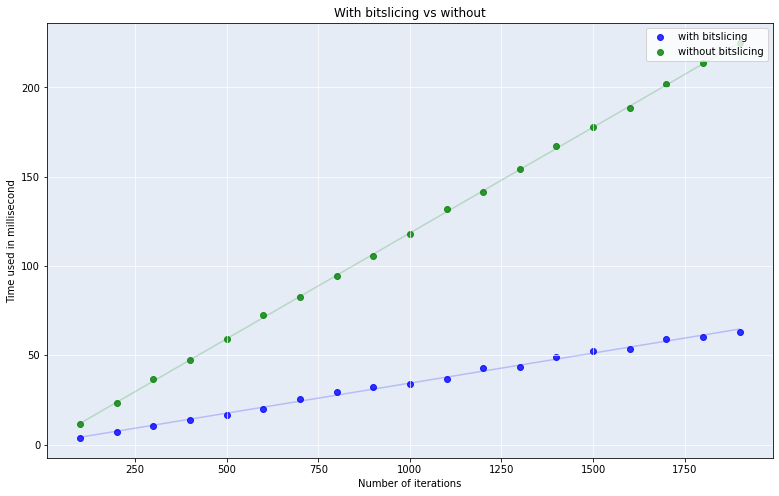
\includegraphics[width=0.75\textwidth]{images/bitslicing_graph_small.png}
\end{figure}
\subsection{Hardware Implementation Performance}
Performance statistics obtained (by authors of RECTANGLE) using implementation in Verilog HDL and Mentor Graphics SE PLUS 6.6d for functional simulation. Hardware designs were synthesized with Synopsys Design Compiler D-2010.03-SP4 to the UMC's 0.13$\mu$m.1P8M low leakage standard cell library with the following values: 1.2V and temperature of 25$\degree$C. Round-based architecture is used which provides direct mapping of the algorithm.\cite{rectangle}\\
Comparing with other lightweight ciphers in \ref{table:compar} we can see that RECTANGLE has a very good throughput per area and per gates used. Also area used in RECTANGLE is given in detail in \ref{table:area}. As expected the S-layer takes low area and the total area is low.(Note: p-layer is just wiring so it's effective area is 0 GE)
\begin{table}[H]
	\centering
	\caption{Area consumption of round-based RECTANGLE 80 and 120}
	\begin{tabular}{|l||l|l|l|l|}
		\hline
&80 bit&&128 bit&\\
\hline
module& Area(GE) & \% & Area(GE) & \% \\ \hline
\hline
data state & 400 & 25.01 & 400 & 19.38\\ \hline
s-layer & 307 & 19.19 & 300 & 14.54\\ \hline
p-layer & 0 & 0 & 0 & 0\\ \hline
key XOR & 176 & 11.00 & 176 & 8.53\\ \hline
key schedule & 713.5 & 44.61 & 1184.5 & 57.4\\ \hline
FSM & 3 & 0.19 & 3 & 0.15\\ \hline
sum & 1599.5 & 100 & 2063.5 & 100\\ \hline
	\end{tabular}
	\label{table:area}
\end{table}

\begin{table}[H]
	\centering
	\caption{Area vs Throughput of different lightweight ciphers}
	\begin{tabular}{|l||l|l|l|l|l|l|}
		\hline
&Key & Block& Cycles& Tech & Area & Throughput\\
&size &size & per Block &($\mu$m) &  & (Kbps)\\ \hline \hline
AES-128 & 128 & 128 & 226 & 0.13 & 2400 & 56.6\\\hline
LED-64 & 64 & 64 & 1248 & 0.18 & 966 & 5.1\\\hline
PICCOLO-80 & 80 & 64 & 27 & 0.13 & 1496 & 237 \\\hline
PRESENT-80 &  80 &  64 & 32 & 0.18 & 1570 & 200 \\\hline
RECTANGLE-80 & 80 &  64 & 26 & 0.13 & 1599.5 & 246 \\\hline
RECTANGLE-128 & 128 & 64 & 26 & 0.13 & 2063.5 & 246 \\
\hline
	\end{tabular}
	\label{table:compar}
\end{table}
\subsection{Software Implementation Performance}
Authors of RECTANGLE implemented RECTANGLE on a 2.5GHz Intel Core i5-2520M CPU - 64 bit C++ compiler and achieved a speed of 30.5cycles/byte.\cite{rectangle}\\
Our implementation of RECTANGLE(unoptimized, Rustc compiler) gave us a good speed and performance. See "implementation" directory for our implementation and timing measurements.
\section{Conclusion}
We have done a survey of lightweight cipher, RECTANGLE. Algorithm, rounds and key schedule of the cipher are covered in detail. An implementation in Rust is also made along with speed measurements. Various observations are made on the design of cipher, Sbox, difference propagation. Linear cryptanalysis and differential cryptanalysis, the most powerful techniques for attacks are covered. Review on performance of RECTANGLE in software and hardware is done. Finally unique aspects of this paper are summarized in Brownie point section.
\section{Brownie Point Nomination}
1. A lot of images are used to help visualize the operations applied.\\
2. Performance comparison of bit-slicing vs normal version is done in software implementation.\\
3. Encryption Algorithm is explained in much more detailed way and is easy to understand.\\
\section{Contribution}
\begin{center}
\begin{tabular}{ |l|l|l| } 
 \hline
   Sl.no. & Task / Area & Members involved\\ \hline \hline
   1& Introduction& Abhiram \& Kausheek\\\hline
   2& The Cipher & Kausheek \& Manu\\\hline
   3& Performance & Manu \& Abhiram \\\hline
   4& Security and Cryptanalysis & All \\\hline
   5& Implementation Bitslicing & Manu \\\hline
   6& Implementation without bitslicing & Kausheek \\\hline
   7& Timing Analysis & Abhiram \\\hline
   8& Term paper - Drawings& All\\\hline
   9&Presentation& All\\ \hline

\end{tabular}
\end{center}

\begin{thebibliography}{9}
\bibitem{rectangle}
Wentao Zhang, Zhenzhen Bao, DongdaiLin, Vincent Rijmen, Bohan Yang, Ingrid Verbauwhede. RECTANGLE: A Bit-slice Lightweight Block CipherSuitable for Multiple Platforms. SCIENCE CHINA Information Sciences, December, 2015, Vol. 58: 122103(15), \href{https://www.doi.org/10.1007/s11432-015-5459-7}{doi: 10.1007/s11432-015-5459-7}


\bibitem{present}
Leander, G.: On Linear Hulls, Statistical Saturation Attacks, PRESENT and a Cryptanalysis of PUFFIN. In:Paterson, K.G. (ed.) EUROCRYPT 2011. LNCS, vol. 6632, pp. 303–322. Springer (2011)


\bibitem{bit1}
Anderson, R., Biham, E., Knudsen, L.R.: Serpent: A Proposal for the Advanced Encryption Standard. NISTAES proposal (1998)

\bibitem{bit2}
Biham, E.: A Fast New DES Implementation in Software. In: Biham, E. (ed.) FSE 1997. LNCS, vol. 1267, pp.260–272. Springer (1997)

\bibitem{iot}
Nordrum, Amy (18 August 2016). "Popular Internet of Things Forecast of 50 Billion Devices by 2020 Is Outdated". \textit{IEEE Spectrum}.

\bibitem{sec}
Singh, Jatinder; Pasquier, Thomas; Bacon, Jean; Ko, Hajoon; Eyers, David (2015). "Twenty Cloud Security Considerations for Supporting the Internet of Things". IEEE Internet of Things Journal. 3 (3): 1 . \href{https://doi.org/10.1109\%2FJIOT.2015.2460333}{doi:10.1109/JIOT.2015.2460333}

\bibitem{imprAttack}
Asuman Senol. Improved Differential Attacks on RECTANGLE. The Graduate School of Informatics of Middle East Technical University. August 2017. \href{http://www.cihangir.forgottenlance.com/files/asuman_senol_master_thesis.pdf}{http://www.cihangir.forgottenlance.com/files/asuman\_senol\_master\_thesis.pdf}
\end{thebibliography}
\end{document}

